% Activate the following line by filling in the right side. If for example the name of the root file is Main.tex, write
% "...root = Main.tex" if the chapter file is in the same directory, and "...root = ../Main.tex" if the chapter is in a subdirectory.
 
%!TEX root =  secondDraft.tex

\chapter[Simulation of Grote Markt]{Simulation of Grote Markt}

In the previous chapter, we have laid out the process from creating a Bayesian Network from a written scenario of a case, and laid out criteria on how to evaluate that network. In this chapter, the method is applied to a simulation of a robbery at the Grote Markt, the main square of Groningen.

By placing agents in a `real' spatial environment, they are constrained by geography in some manner - they cannot see through buildings, and cannot move through them. These affordances result in more interesting behaviours for the agents, and are a first step towards using this approach to less abstracted societal issues.



\section{Scenario}
There are two agents walking around the area of Grote Markt. One of the agents is old and carries a valuable object. The other agent is young, and might potentially steal the object. If the potential thief sees the potential victim, it decides whether the potential victim is vulnerable enough to steal from, and the object is valuable enough. If both of these conditions are fulfilled, the agent becomes a potential thief, and now has a motive to steal from the old agent. The agent will attempt to sneak up on the victim, and steal the object from the old agent. At some point, the old agent realises that their valuable object is gone. This is the first scenario. In the second scenario, the old agent simply dropped the valuable object, and after a while notices that it is gone. As evidence, we have a psychological report that estimates whether the young agent is capable of the crime, we might have video footage of the thief stealing the object, and we have the fact that the potential thief shows up on camera. 

Additionally, outside the described scenario, we also have access to the `mental' state of the potential thief, so we know whether they actually consider the old agent vulnerable, and whether they find the object itself valuable. We also know if the thief is actually intending to sneak up on the other agent.


\section{Simulation}

We extract the relevant agents from the scenario, we need two of them: a potential thief, and a potential victim. Every agent has an age, to determine whether they are vulnerable or not - old people are considered more vulnerable. Every agent also has an object of a certain value, the thief's object has a value of -1, and the other agent's object has a value of 1000, to make it a tempting target. An agent decides if it wants to steal something by making a very simple risk-calculation based on their risk threshold: if the object is more expensive than their risk threshold, they will attempt to steal it (contributing to `motive'). Every agent also has a goal state, this is the location at the edge of the map. When they enter their goal state, they are essentially removed from the simulation, as they leave the relevant area. Every simulation was run for 100 timesteps, or until both agents are in their goal states. The simulation itself was ran 500 times. The behaviour of the agents is shown in Figure~\ref{behaviourGM}. Agents are placed randomly on the map.

The operationalisation of the random variables is described below. The output node is the node `stealing\_1\_0':
\begin{description}


\item[seen\_1\_0  ] if the victim agent is in the line of sight of the thief agent.
\item[know\_valuable\_1\_0 ] if the value is higher than the risk threshold.
\item[know\_vulnerable\_1\_0  ] if the victim's age is older than the thief's threshold age.
\item[motive\_1\_0 ] if the object is more valuable than the risk threshold, the victim's age is older than the thief's threshold age, and the thief is not already stealing from someone else. 
\item[sneak\_1\_0 ] if the thief has targeted the victim (has a motive) , but is not yet in the same position.
\item[stealing\_1\_0 ] if the thief has targeted the victim, the object's value is greater than the risk threshold, and the thief's position is the same as the victim's position. 
\item[object\_dropped\_accidentally\_0 ] at every epoch, there is a 1/500 probability that the victim agent will drop the object by accident.
\item[E\_vulnerable\_1\_0 ] the thief decides that the target is vulnerable (know\_vulnerable\_1\_0 is true).
\item[E\_valuable\_1\_0 ] the thief decides that the object is valuable (know\_valuable\_1\_0 is true).
\item[E\_sneak\_1\_0 ] the agent sneaks up on the target (sneak\_1\_0 is true).
\item[E\_camera\_1 ] the thief is seen on any one of the cameras.
\item[E\_psych\_report\_1\_0 ] if the thief has a motive, we draw an estimated risk threshold and an estimated age threshold from two normal distributions (mean = victim age, sd = 20), (mean = value good, sd = 100). If the victim is older than the thief's minimal age threshold, and the object more valuable, we estimate that the psych profile states that the victim fits the thief's profile, else not.
\item[E\_camera\_1 ] the thief is seen on any one of the cameras.
\item[E\_object\_gone\_0 ] if the object is dropped accidentally, or if the object has been stolen.
\item[E\_camera\_seen\_stealing\_1\_0 ]  if any camera sees the thief during the state in which it is stealing.
\end{description}

The environment for the agents was created by converting a map image into an agent-readable world. This was done by writing a method to convert screenshots of maps into an agent-readable environment. The maps were screenshotted from \url{http://maps.stamen.com/terrain/#18/53.21618/6.57225} and converted into greyscale. Then, they were transformed into a grid of a given size. The average greyscale value of each cell in the grid was taken and coded as either `accessible' or `non-accessible'. On the greyscale map, the color of the buildings was in the range of (189, 199) - cells within this range were coded as `inaccessible', since agents cannot walk through buildings. All other cells were `accessible'. This resulted in a map shared by all agents that constrained their movements. There are 5 cameras placed randomly on the `accessible' cells on the map, each with a visual radius of 8. Additionally, we used this map to calculate the sight lines of both cameras and agents. An agent or a camera cannot see another agent if there is an `inaccessible' grid cell on the sight line between the two.



\begin{figure}[htbp]
\begin{center}
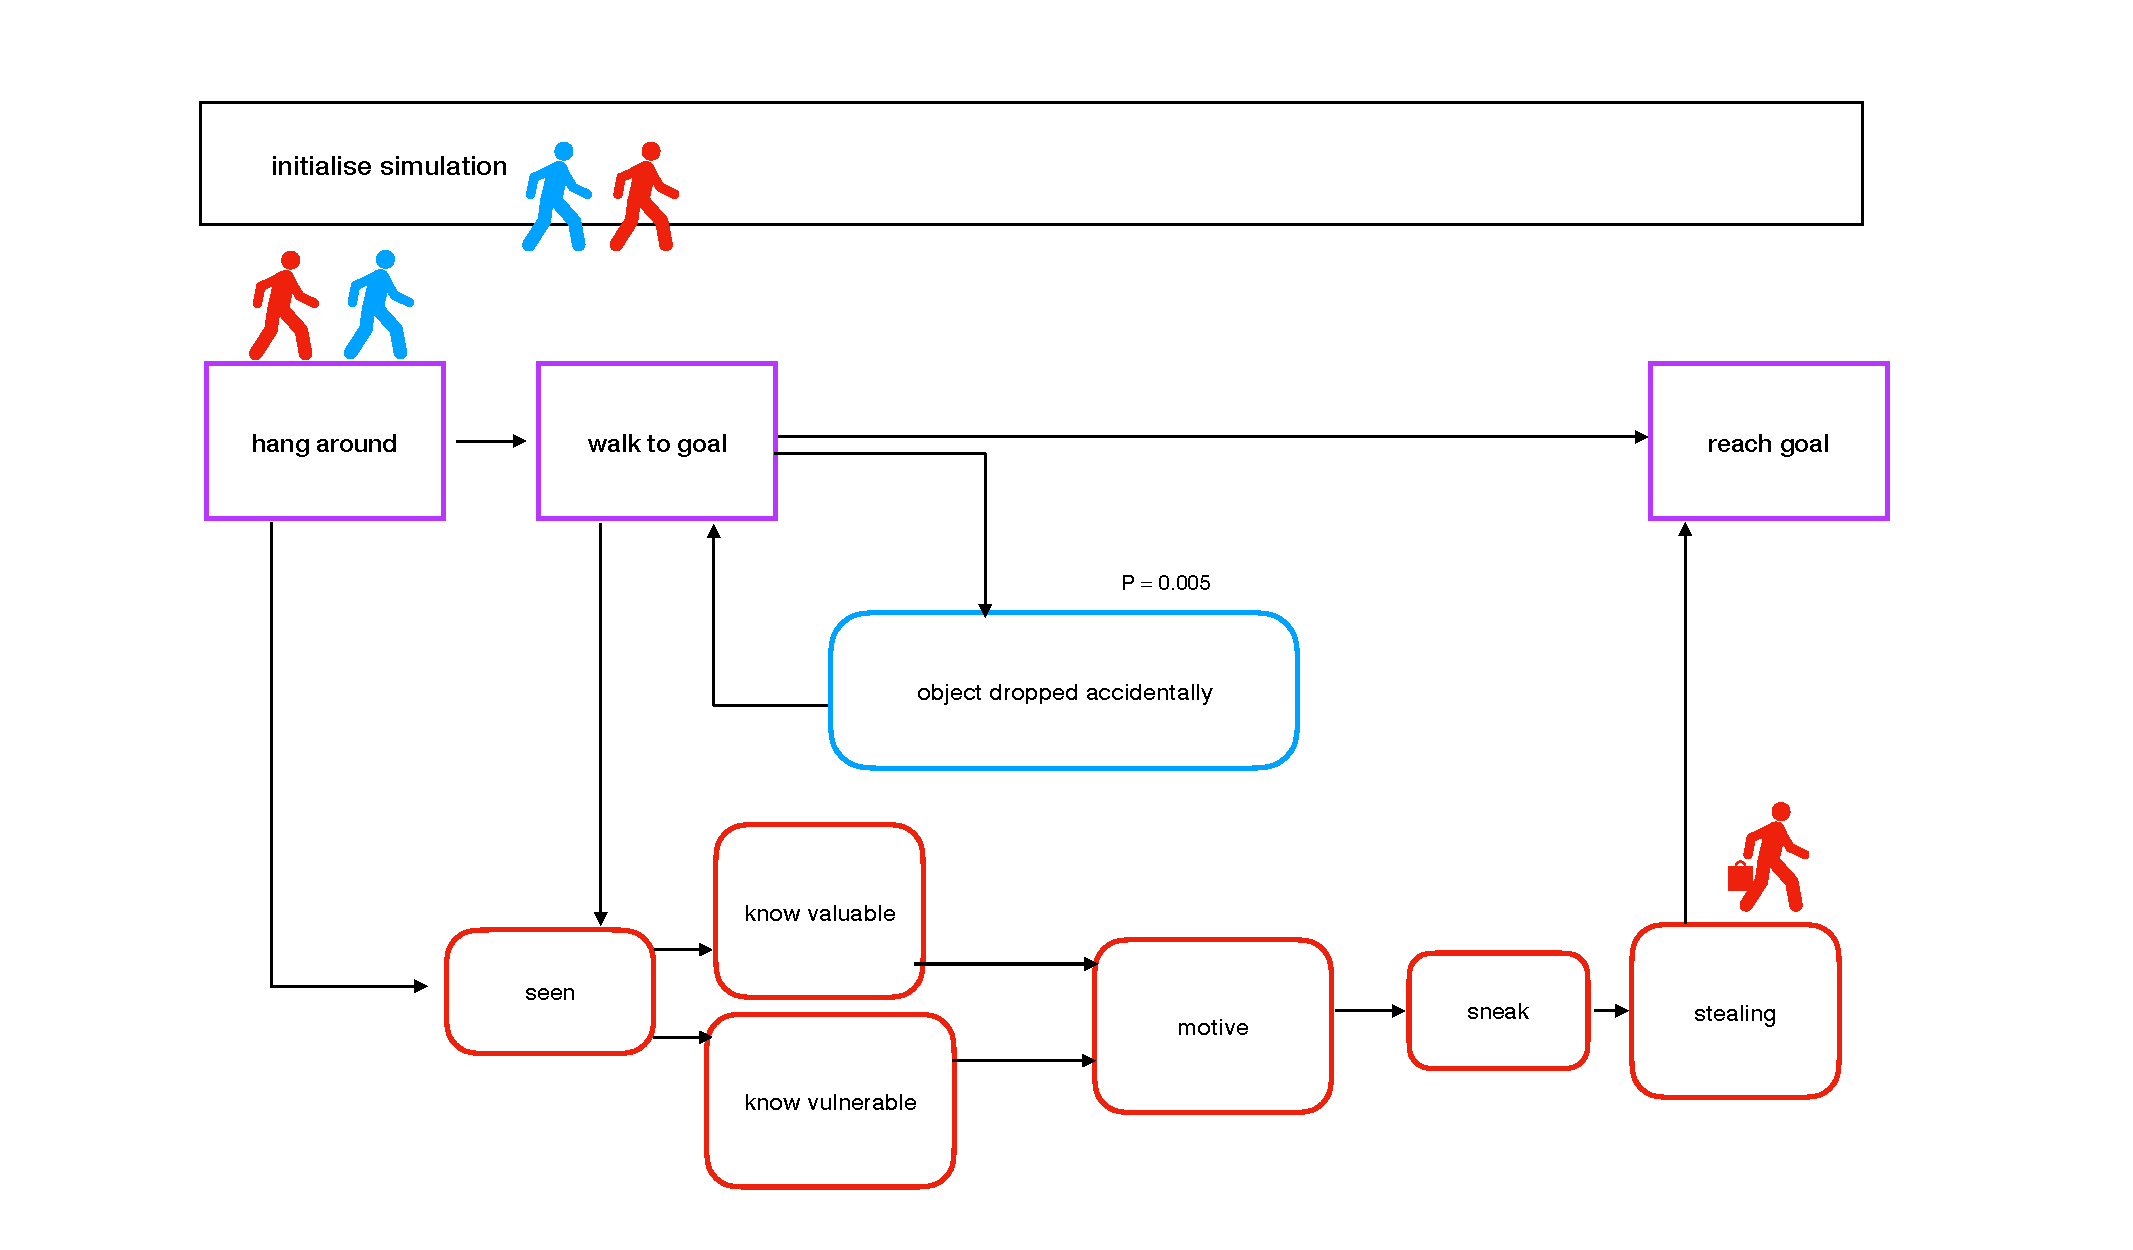
\includegraphics[width=\linewidth]{images/grotemarkt.pdf}
\end{center}
\caption{The behaviour of the agents. The nodes with rounded edges correspond to the nodes in the Bayesian Network.}
\label{behaviourGM}
\end{figure}


\begin{figure}[htbp]
\begin{center}
\begin{subfigure}{.5\textwidth}
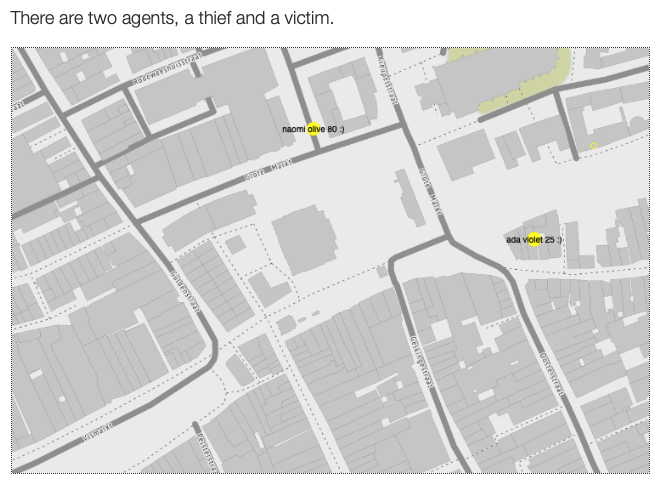
\includegraphics[width=\linewidth]{images/grotemarktmap.png}
\caption{map of environment - 2 agents}
\end{subfigure}%
\begin{subfigure}{.5\textwidth}
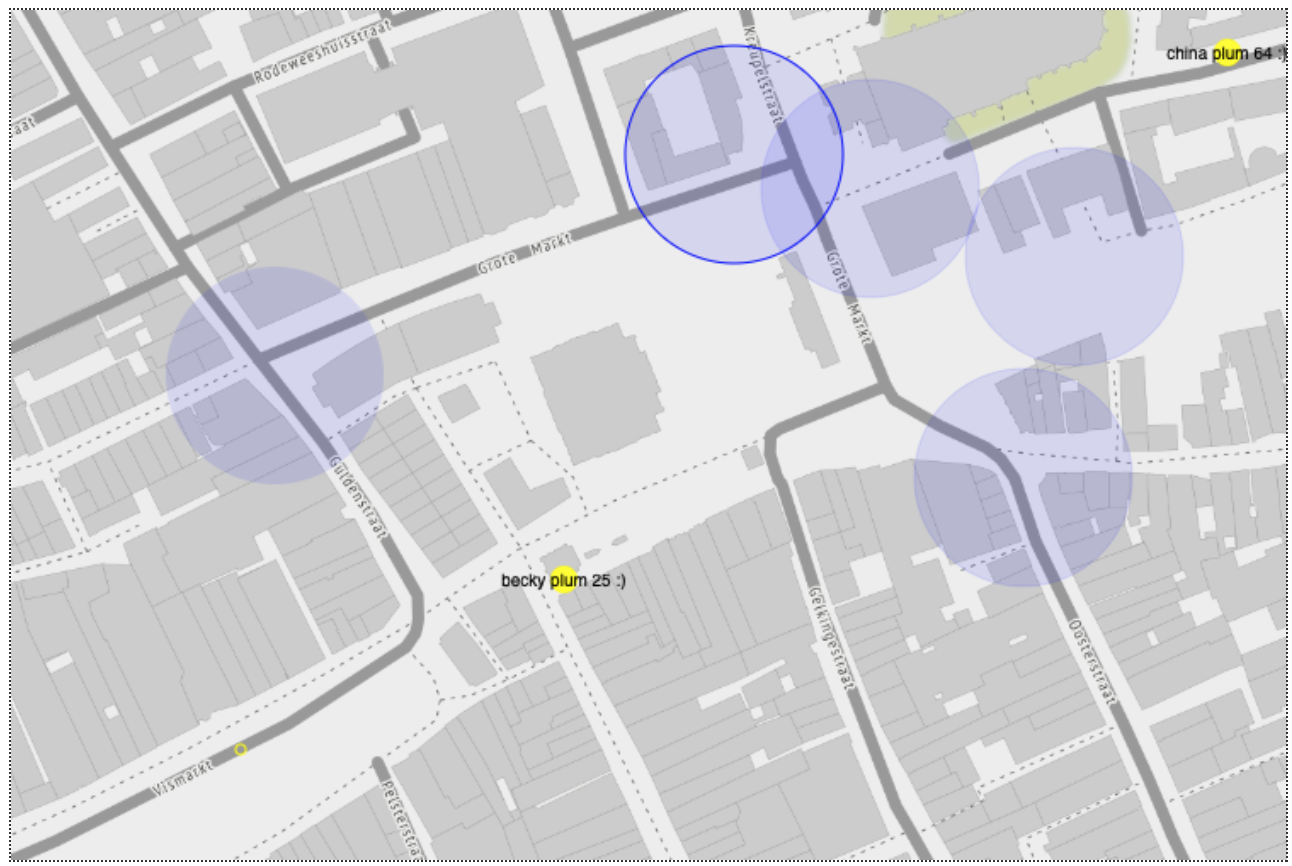
\includegraphics[width=\linewidth]{images/agentGM.png}
\caption{Camera locations are randomly initialized}
\end{subfigure}%
\label{groteMarkt}
\caption{The Grote Markt environment}
\end{center}
\end{figure}





\section{Network}

The network is shown in Figure~\ref{wedding}.

\begin{figure}
\begin{center}
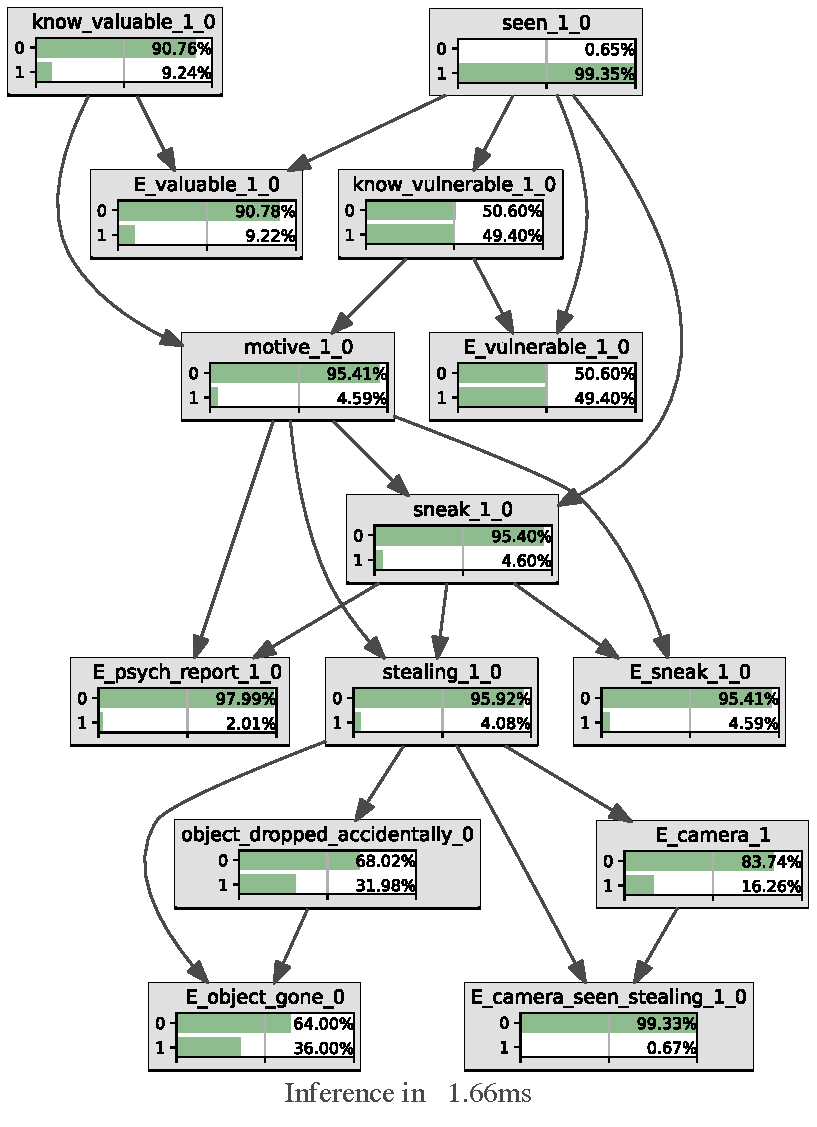
\includegraphics[width=1.2\linewidth]{../experiments/GroteMarkt/bnImage/BNIMAGEGroteMarkt.pdf}
\caption{Network of Grote Markt simulation.}
\label{wedding}
\end{center}
\end{figure}


\section{Evaluation}



\subsection{Numbers}
\begin{enumerate}
\item \textbf{The conditional frequencies in the BN correspond to the conditional frequencies in the simulation}
\item \textbf{The values in the conditional probability tables are elicitable from human modellers}
\item \textbf{The BN is robust against imprecision in the conditional probability tables}
\end{enumerate}

\subsection{Structural}

\begin{enumerate}
\item \textbf{The BN represents all events of the scenario}
\item \textbf{The BN has temporal ordering of the hypothesis nodes}
\item \textbf{The BN follows the evidence-idiom}
\item \textbf{The BN represents multiple alternative scenarios}

\end{enumerate}

\subsection{Predictive Skills}
\begin{enumerate}
\item \textbf{The BN only predicts high probability of the output node given relevant evidence truth values}

\begin{figure}[htbp]
\begin{center}
\begin{subfigure}{.66\textwidth}
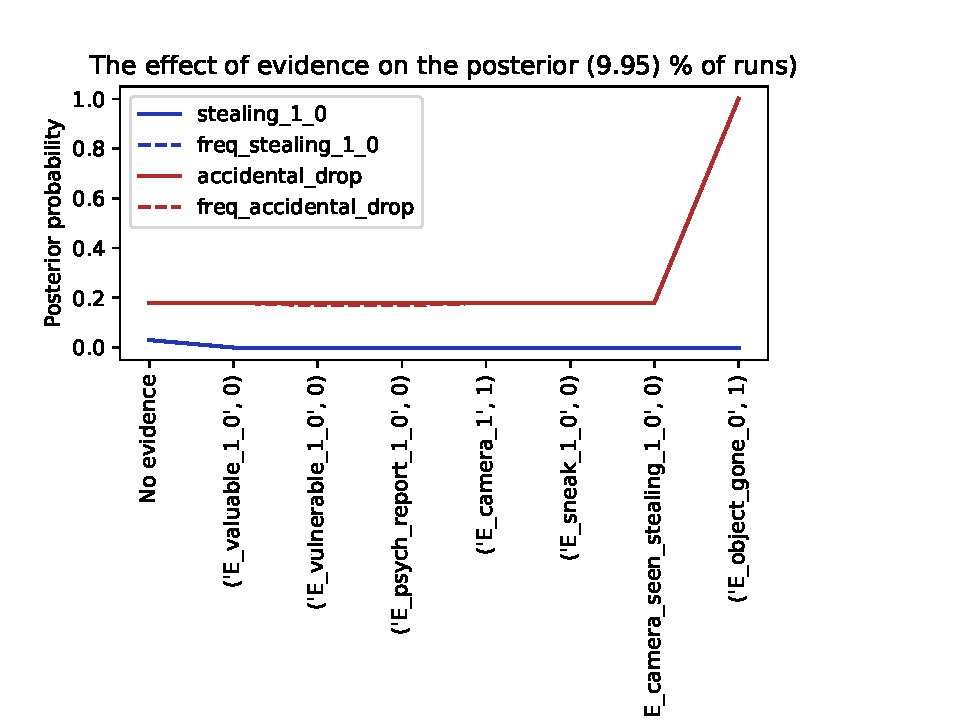
\includegraphics[width=\linewidth]{../experiments/GroteMarkt/plots/evidence_progress_GroteMarkt_2.pdf}
\caption{All evidence is true.}
\label{default}
\end{subfigure}%
\begin{subfigure}{.66\textwidth}
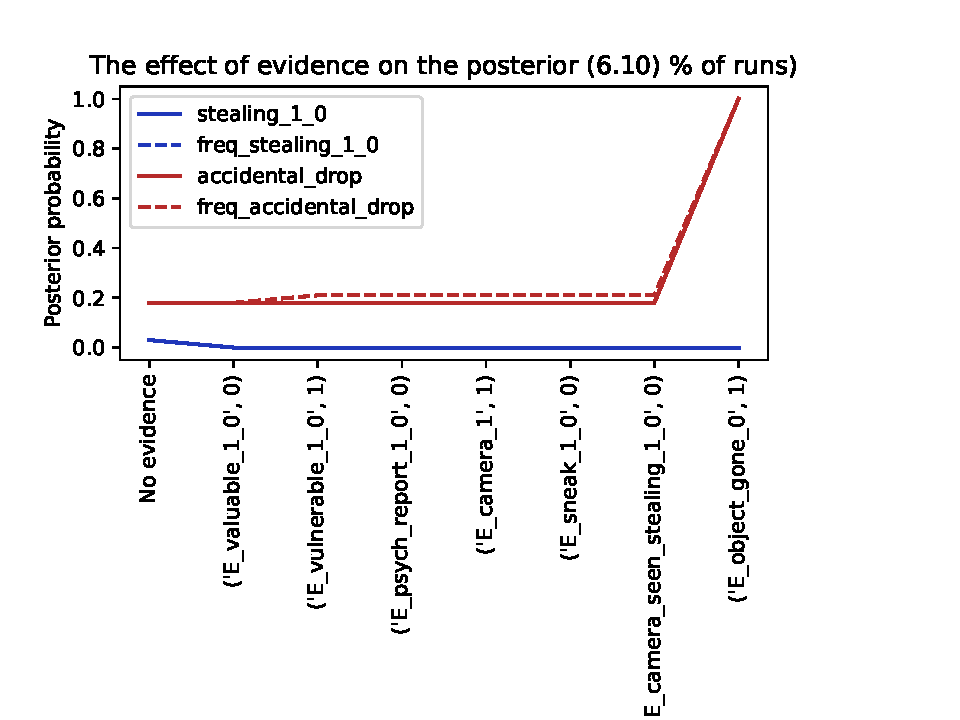
\includegraphics[width=\linewidth]{../experiments/GroteMarkt/plots/evidence_progress_GroteMarkt_1.pdf}
\caption{Agent only has assessed vulnerable.}
\label{default}
\end{subfigure}
\begin{subfigure}{.66\textwidth}
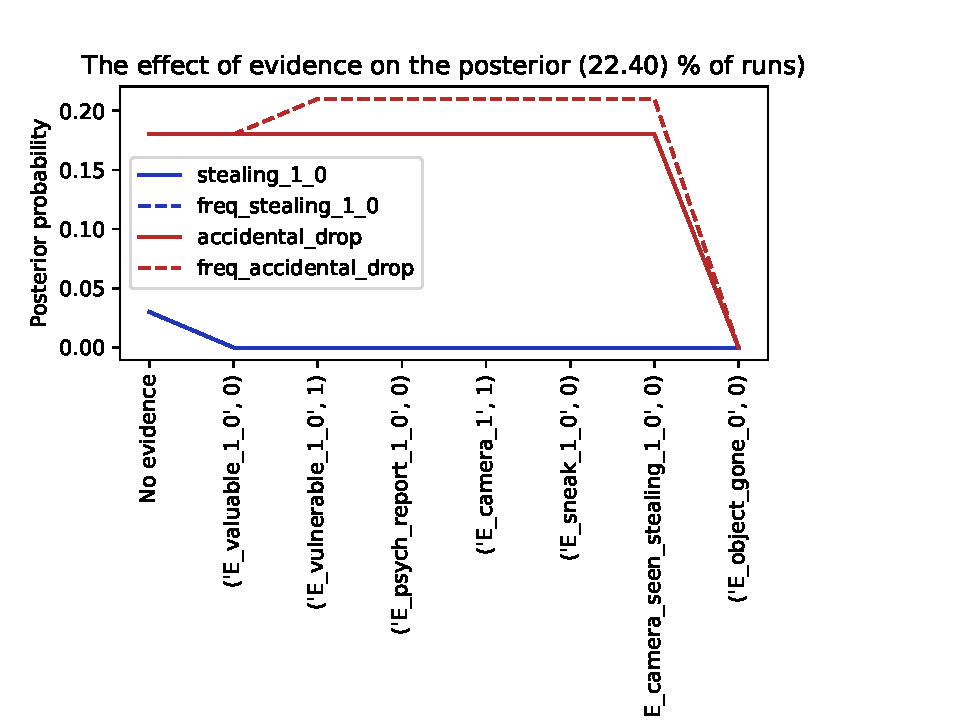
\includegraphics[width=\linewidth]{../experiments/GroteMarkt/plots/evidence_progress_GroteMarkt_3.pdf}
\caption{Agent was only seen on camera.}
\label{default}
\end{subfigure}%
\begin{subfigure}{.66\textwidth}
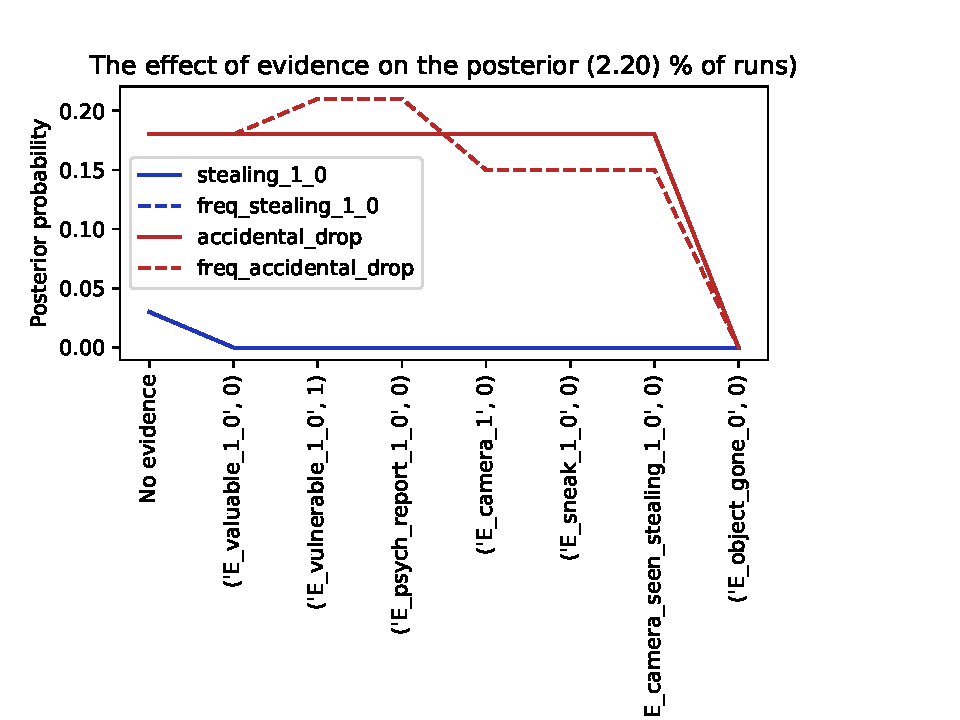
\includegraphics[width=\linewidth]{../experiments/GroteMarkt/plots/evidence_progress_GroteMarkt_4.pdf}
\caption{Agent was seen on camera and object is gone.}
\label{default}
\end{subfigure}
\caption{Effect of evidence on posterior.}
\label{malthus}
\end{center}
\end{figure}

We see here that the posterior probability of the `stealing\_1\_0' node reflects exculpatory evidence well - as soon as we find evidence that would make it impossible for the agent to have stolen (such as not finding the other agent vulnerable, or the object valuable), the posterior for stealing immediately turns to 0. 

However, if we look at the progression of evidence in 4.4(a), where all the evidence is true, we see a posterior $>0.9$ for the `stealing\_1\_0' node as soon as we entered that the agent has a motive (`E\_psych\_report'). Depending on a given guilt threshold, this might be enough to convict. But this is very weak evidence in real life - just because the agent might have a motive, does not mean that it is going to steal. We see a small increase in the posterior when `E\_camera\_seen\_stealing\_1\_0' is set to true, when this should really be the strongest piece of evidence in the entire set. This shows that if we have access to the private knowledge of the agent (its intention to steal), we can make good predictions.


\item \textbf{We can know when the BN predicts the wrong outcome}
\end{enumerate}

\section{Discussion}


\subsection{Problems}
\begin{enumerate}
\item \textbf{Does the BN not depend on private knowledge?}
\item \textbf{Could we apply this BN to a different location? }
\item \textbf{Identity and guilt?}

\end{enumerate}


\subsection{Legal Interpretation}



